\documentclass[titlepage]{article}
\usepackage{listings}
\lstMakeShortInline{|}
\usepackage{courier}
%\usepackage{hyperref}
\usepackage[colorlinks,linkcolor=blue,citecolor=blue,urlcolor=blue,breaklinks=true]{hyperref}
\lstset{basicstyle=\ttfamily\small , breaklines}
%\usepackage[margin=2cm]{geometry}
\usepackage[left=3cm,top=3cm,bottom=3cm, right=3cm,includehead,includefoot,landscape]{geometry}
\usepackage{color}
\usepackage{fancyhdr,lastpage}
\pagestyle{fancy}
\rhead{Metrum Research Group, LLC \\ }
\lhead{
\includegraphics[scale=2]{logo.png}}
\cfoot{Page \thepage\ of \pageref{LastPage}}
\fancyhfoffset{.25in}
\renewcommand{\headrulewidth}{0.25pt}
\renewcommand{\footrulewidth}{0pt} 
\setlength{\headheight}{23pt}
\renewcommand{\labelitemiii}{$\circ$}
\usepackage{longtable}
\usepackage{amsmath}
\usepackage[T1]{fontenc}
\usepackage[scaled]{helvet}
\renewcommand*\familydefault{\sfdefault}
\usepackage{courier}
\usepackage{graphicx}
\usepackage{tocbibind}
\usepackage[parfill]{parskip}    % Activate to begin paragraphs with an empty line rather than an indent
\usepackage{upgreek}
\usepackage{textpos}
\usepackage{relsize}
\usepackage{upquote}
% Use \begin{landscape} and end{landscape} to rotate text %%%
\usepackage{pdflscape}
\usepackage{textcomp}
\usepackage{float}
\floatplacement{figure}{H}
\floatplacement{table}{H}
\usepackage[printonlyused,nohyperlinks]{acronym}
\def\bflabel#1{{\large#1\ \ \ \ }\hfill}
\usepackage{fixltx2e}
\setlength{\belowcaptionskip}{10pt}





\usepackage{Sweave}

 
\begin{document}
\vspace*{2cm}
\begin{center}
{\Large MIfuns Sample Script}\\
\vspace{1.5cm}
{\Large Phase I Modeling}\\
~\\
\today\\
~\\
Tim Bergsma\\
\end{center}
\newpage

\section{Purpose}
This script runs NONMEM models and diagnostics for sample phase1 data.
\section{Model Development}
\subsection{Set up for NONMEM run.}
\begin{Schunk}
\begin{Sinput}
> getwd()
\end{Sinput}
\begin{Soutput}
[1] "/Users/timb/project/metrum-mifuns/inst/sample/script"
\end{Soutput}
\begin{Sinput}
> library(MIfuns)
\end{Sinput}
\begin{Soutput}
MIfuns 4.0.11 loaded
Installing SIGCHLD signal handler...Done.
\end{Soutput}
\begin{Sinput}
> command <- '/common/NONMEM/nm7_osx1/test/nm7_osx1.pl'
> cat.cov='SEX'
> cont.cov=c('HEIGHT','WEIGHT','AGE')
> par.list=c('CL','Q','KA','V','V2','V3')
> eta.list=paste('ETA',1:10,sep='')
\end{Sinput}
\end{Schunk}
\subsection{Run NONMEM.}
To force a re-run of this model, delete 1005/diagnostics.pdf.
\begin{Schunk}
\begin{Sinput}
> if(!file.exists('../nonmem/1005/diagnostics.pdf'))NONR(
+      run=1005,
+      command=command,
+      project='../nonmem',
+      grid=TRUE,
+      nice=TRUE,
+      checkrunno=FALSE,
+      cont.cov=cont.cov,
+      cat.cov=cat.cov,
+      par.list=par.list,
+      eta.list=eta.list,
+      plotfile='../nonmem/*/diagnostics.pdf',
+      streams='../nonmem/ctl'
+ )
> getwd()
\end{Sinput}
\begin{Soutput}
[1] "/Users/timb/project/metrum-mifuns/inst/sample/script"
\end{Soutput}
\begin{Sinput}
> while(!file.exists('../nonmem/1005/diagnostics.pdf')){}
\end{Sinput}
\end{Schunk}
Covariance succeeded on model 1005.
\section{Predictive Check}
\subsection{Create a simulation control stream.}
\begin{Schunk}
\begin{Sinput}
> t <- metaSub(
+      as.filename('../nonmem/ctl/1005.ctl'),
+      names=1105,
+      pattern=c(
+          '\\$THETA[^$]+',
+          '\\$OMEGA[^$]+',
+          '\\$SIGMA[^$]+',
+          '\\$EST[^$]+',
+          '\\$COV',
+          '\\$TABLE.*'
+      ),
+      replacement=c(
+          '$MSFI=../1005/1005.msf\n',
+          ';$OMEGA\n',
+          ';$SIGMA\n',
+          '$SIMULATION ONLYSIM (1968) SUBPROBLEMS=500\n',
+          ';$COV',
+          '$TABLE DV NOHEADER NOPRINT FILE=./*.tab FORWARD NOAPPEND\n'
+     ),
+     fixed=FALSE,
+     out='../nonmem/ctl',
+     suffix='.ctl'
+ )
\end{Sinput}
\end{Schunk}
\subsection{Run the simulation.}
This run makes the predictions (simulations).
\begin{Schunk}
\begin{Sinput}
> if(!file.exists('../nonmem/1105/1105.lst'))NONR(
+      run=1105,
+      command=command,
+      project='../nonmem',
+      grid=TRUE,
+      nice=TRUE,
+      diag=FALSE,
+      streams='../nonmem/ctl'
+ )
> getwd()
\end{Sinput}
\begin{Soutput}
[1] "/Users/timb/project/metrum-mifuns/inst/sample/script"
\end{Soutput}
\begin{Sinput}
> while(!file.exists('../nonmem/1105/1105.lst')){}
\end{Sinput}
\end{Schunk}
\subsection{Recover and format the original dataset.}
Now we fetch the results and integrate them with the other data.
\begin{Schunk}
\begin{Sinput}
> phase1 <- read.csv('../data/derived/phase1.csv',na.strings='.')
> head(phase1)
\end{Sinput}
\begin{Soutput}
     C ID TIME SEQ EVID  AMT    DV SUBJ HOUR TAFD  TAD LDOS MDV HEIGHT WEIGHT
1    C  1 0.00   0    0   NA 0.000    1 0.00 0.00   NA   NA   0    174   74.2
2 <NA>  1 0.00   1    1 1000    NA    1 0.00 0.00 0.00 1000   1    174   74.2
3 <NA>  1 0.25   0    0   NA 0.363    1 0.25 0.25 0.25 1000   0    174   74.2
4 <NA>  1 0.50   0    0   NA 0.914    1 0.50 0.50 0.50 1000   0    174   74.2
5 <NA>  1 1.00   0    0   NA 1.120    1 1.00 1.00 1.00 1000   0    174   74.2
6 <NA>  1 2.00   0    0   NA 2.280    1 2.00 2.00 2.00 1000   0    174   74.2
  SEX  AGE DOSE FED SMK DS CRCN predose zerodv
1   0 29.1 1000   1   0  0 83.5       1      1
2   0 29.1 1000   1   0  0 83.5       0      0
3   0 29.1 1000   1   0  0 83.5       0      0
4   0 29.1 1000   1   0  0 83.5       0      0
5   0 29.1 1000   1   0  0 83.5       0      0
6   0 29.1 1000   1   0  0 83.5       0      0
\end{Soutput}
\begin{Sinput}
> phase1 <- phase1[is.na(phase1$C),c('SUBJ','TIME','DV')]
> records <- nrow(phase1)
> records
\end{Sinput}
\begin{Soutput}
[1] 550
\end{Soutput}
\begin{Sinput}
> phase1 <- phase1[rep(1:records,500),]
> nrow(phase1)
\end{Sinput}
\begin{Soutput}
[1] 275000
\end{Soutput}
\begin{Sinput}
> phase1$SIM <- rep(1:500,each=records)
> #head(phase1,300)
> with(phase1,DV[SIM==1 & SUBJ==12])
\end{Sinput}
\begin{Soutput}
 [1]     NA  2.260  2.830  8.730 19.300 15.200 16.200  8.830 12.900 12.700
[11]  7.140  5.740  1.980  0.791
\end{Soutput}
\begin{Sinput}
> with(phase1,DV[SIM==2 & SUBJ==12])
\end{Sinput}
\begin{Soutput}
 [1]     NA  2.260  2.830  8.730 19.300 15.200 16.200  8.830 12.900 12.700
[11]  7.140  5.740  1.980  0.791
\end{Soutput}
\end{Schunk}
\subsection{Recover and format the simulation results.}
\begin{Schunk}
\begin{Sinput}
> pred <- scan('../nonmem/1105/1105.tab')
> nrow(phase1)
\end{Sinput}
\begin{Soutput}
[1] 275000
\end{Soutput}
\begin{Sinput}
> length(pred)
\end{Sinput}
\begin{Soutput}
[1] 275000
\end{Soutput}
\end{Schunk}
\subsection{Combine the original data and the simulation data.}
\begin{Schunk}
\begin{Sinput}
> phase1$PRED <- pred
> head(phase1)
\end{Sinput}
\begin{Soutput}
  SUBJ TIME    DV SIM    PRED
2    1 0.00    NA   1 0.00000
3    1 0.25 0.363   1 0.17932
4    1 0.50 0.914   1 0.53642
5    1 1.00 1.120   1 0.78983
6    1 2.00 2.280   1 1.84990
7    1 3.00 1.630   1 1.96530
\end{Soutput}
\begin{Sinput}
> phase1 <- phase1[!is.na(phase1$DV),]
> head(phase1)
\end{Sinput}
\begin{Soutput}
  SUBJ TIME    DV SIM    PRED
3    1 0.25 0.363   1 0.17932
4    1 0.50 0.914   1 0.53642
5    1 1.00 1.120   1 0.78983
6    1 2.00 2.280   1 1.84990
7    1 3.00 1.630   1 1.96530
8    1 4.00 2.040   1 2.01810
\end{Soutput}
\end{Schunk}
\subsection{Plot predictive checks.}
\subsubsection{Aggregate data within subject.}
Since subjects may contribute differing numbers of observations, it may
be useful to look at predictions from a subject-centric perspective.
Therefore, we wish to calculate summary statistics for each subject, 
(observed and predicted) and then make obspred comparisons therewith.
\begin{Schunk}
\begin{Sinput}
> library(reshape)
> head(phase1)
\end{Sinput}
\begin{Soutput}
  SUBJ TIME    DV SIM    PRED
3    1 0.25 0.363   1 0.17932
4    1 0.50 0.914   1 0.53642
5    1 1.00 1.120   1 0.78983
6    1 2.00 2.280   1 1.84990
7    1 3.00 1.630   1 1.96530
8    1 4.00 2.040   1 2.01810
\end{Soutput}
\begin{Sinput}
> subject <- melt(phase1,measure.var=c('DV','PRED'))
> head(subject)
\end{Sinput}
\begin{Soutput}
  SUBJ TIME SIM variable value
1    1 0.25   1       DV 0.363
2    1 0.50   1       DV 0.914
3    1 1.00   1       DV 1.120
4    1 2.00   1       DV 2.280
5    1 3.00   1       DV 1.630
6    1 4.00   1       DV 2.040
\end{Soutput}
\end{Schunk}
We are going to aggregate each subject's DV and PRED values using cast().
cast() likes an aggregation function that returns a list.
We write one that grabs min med max for each subject, sim, and variable.
\begin{Schunk}
\begin{Sinput}
> metrics <- function(x)list(min=min(x), med=median(x), max=max(x))
\end{Sinput}
\end{Schunk}
Now we cast, ignoring time.
\begin{Schunk}
\begin{Sinput}
> subject <- data.frame(cast(subject, SUBJ + SIM + variable ~ .,fun=metrics))
> head(subject)
\end{Sinput}
\begin{Soutput}
  SUBJ SIM variable      min    med    max
1    1   1       DV 0.363000 1.6100 3.0900
2    1   1     PRED 0.179320 1.9653 5.0314
3    1   2       DV 0.363000 1.6100 3.0900
4    1   2     PRED 0.096462 3.0448 7.4728
5    1   3       DV 0.363000 1.6100 3.0900
6    1   3     PRED 0.450430 5.5284 8.7665
\end{Soutput}
\end{Schunk}
Note that regardless of SIM, DV (observed) is constant.

Now we melt the metrics.
\begin{Schunk}
\begin{Sinput}
> metr <- melt(subject,measure.var=c('min','med','max'),variable_name='metric')
> head(metr)
\end{Sinput}
\begin{Soutput}
  SUBJ SIM variable metric    value
1    1   1       DV    min 0.363000
2    1   1     PRED    min 0.179320
3    1   2       DV    min 0.363000
4    1   2     PRED    min 0.096462
5    1   3       DV    min 0.363000
6    1   3     PRED    min 0.450430
\end{Soutput}
\end{Schunk}
\subsubsection{Aggregate data across subjects, within simulations.}
Our predictions have central tendencies, which can vary by SIM.
Thus, our metrics as well have central tendencies that vary by SIM.
We want to represent the variability across SIMS by aggregating within SIM.
That means aggregating across subjects, within SIMS.  
There are many aggregation strategies, but we choose quantiles for a non-parametric 
result. Quantiles that 'clip' the tails of the distribution offer robustness against
number of SIMS (i.e., results less dependent on number of sims).  
Within each SIM, let's find for each metric the 5th, 50th, and 95th percentile.
We also want to do this for the original data set (requires some minor rearrangement).
\begin{Schunk}
\begin{Sinput}
> head(metr)
\end{Sinput}
\begin{Soutput}
  SUBJ SIM variable metric    value
1    1   1       DV    min 0.363000
2    1   1     PRED    min 0.179320
3    1   2       DV    min 0.363000
4    1   2     PRED    min 0.096462
5    1   3       DV    min 0.363000
6    1   3     PRED    min 0.450430
\end{Soutput}
\begin{Sinput}
> quants <- data.frame(cast(metr,SIM + metric + variable ~ .,fun=quantile,probs=c(0.05,0.50,0.95)))
> head(quants,10)
\end{Sinput}
\begin{Soutput}
   SIM metric variable       X5.    X50.     X95.
1    1    min       DV 0.3054500  2.1450  36.0750
2    1    min     PRED 0.0976828  2.3129  29.6127
3    1    med       DV 1.5860000 20.2500 290.2000
4    1    med     PRED 2.2552400 22.8675 304.0180
5    1    max       DV 3.0855000 40.7000 634.2500
6    1    max     PRED 4.4729900 47.2865 579.6585
7    2    min       DV 0.3054500  2.1450  36.0750
8    2    min     PRED 0.0949232  2.8080  32.3266
9    2    med       DV 1.5860000 20.2500 290.2000
10   2    med     PRED 1.6609825 23.4225 263.8535
\end{Soutput}
\end{Schunk}
Note, again, that DV quantiles are invariant across SIMS.
\subsubsection{Reformat data for bivariate display.}
We now have a lot of display options.  The simplest is to plot DV~PRED for each quantile and metric.
Requires slight rearrangement.
\begin{Schunk}
\begin{Sinput}
> molten <- melt(quants, measure.var=c('X5.','X50.','X95.'),variable_name='quant')
> head(molten)
\end{Sinput}
\begin{Soutput}
  SIM metric variable quant     value
1   1    min       DV   X5. 0.3054500
2   1    min     PRED   X5. 0.0976828
3   1    med       DV   X5. 1.5860000
4   1    med     PRED   X5. 2.2552400
5   1    max       DV   X5. 3.0855000
6   1    max     PRED   X5. 4.4729900
\end{Soutput}
\begin{Sinput}
> frozen <- data.frame(cast(molten, SIM + metric + quant ~ variable))
> head(frozen)
\end{Sinput}
\begin{Soutput}
  SIM metric quant        DV        PRED
1   1    min   X5.   0.30545   0.0976828
2   1    min  X50.   2.14500   2.3129000
3   1    min  X95.  36.07500  29.6127000
4   1    med   X5.   1.58600   2.2552400
5   1    med  X50.  20.25000  22.8675000
6   1    med  X95. 290.20000 304.0180000
\end{Soutput}
\end{Schunk}
\subsubsection{Bivariate display of within-simulation aggregate metrics.}
\begin{Schunk}
\begin{Sinput}
> print(xyplot(
+ 	log(PRED)~log(DV)|metric,
+ 	frozen,
+ 	groups=quant,
+ 	layout=c(1,3),
+ 	auto.key=TRUE,
+ 	panel=function(...){
+ 		panel.xyplot(...)
+ 		panel.abline(a=0,b=1)
+ 	}
+ ))
\end{Sinput}
\end{Schunk}
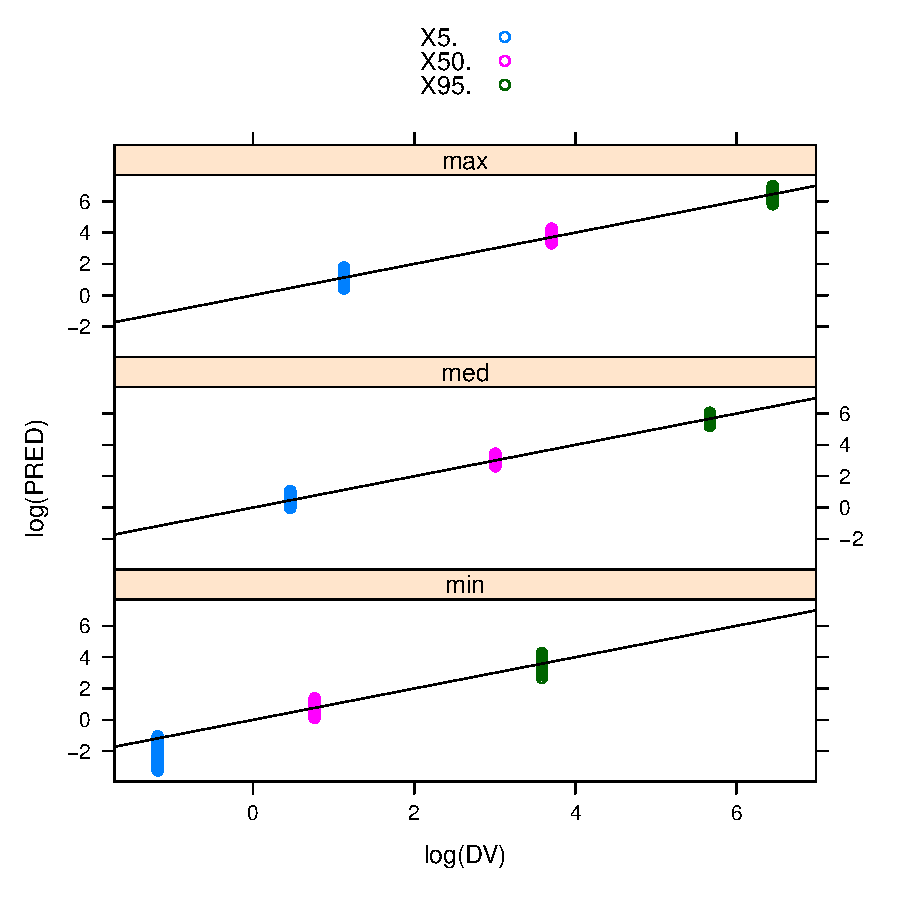
\includegraphics{model-bivariate}
\subsubsection{Univariate displays.}
For a better view of the distributions, however, we can work with single-axis plot functions,
using the molten data.  For faster and clearer plotting, we remove duplicates of DV.
\subsubsection{Classic stripplot}
\begin{Schunk}
\begin{Sinput}
> head(molten)
\end{Sinput}
\begin{Soutput}
  SIM metric variable quant     value
1   1    min       DV   X5. 0.3054500
2   1    min     PRED   X5. 0.0976828
3   1    med       DV   X5. 1.5860000
4   1    med     PRED   X5. 2.2552400
5   1    max       DV   X5. 3.0855000
6   1    max     PRED   X5. 4.4729900
\end{Soutput}
\begin{Sinput}
> molten$SIM <- NULL
> table(molten$variable)
\end{Sinput}
\begin{Soutput}
  DV PRED 
4500 4500 
\end{Soutput}
\begin{Sinput}
> molten <- molten[!(duplicated(molten[,c('metric','variable','quant')]) & molten$variable=='DV'),]
> table(molten$variable)
\end{Sinput}
\begin{Soutput}
  DV PRED 
   9 4500 
\end{Soutput}
\begin{Sinput}
> library(grid)
> print(stripplot(
+ 	~value|metric+quant,
+ 	molten,
+ 	groups=variable,
+ 	horizontal=TRUE,
+ 	auto.key=TRUE,
+ 	panel=panel.superpose,
+ 	alpha=0.5,
+ 	panel.groups=panel.stripplot
+ ))
\end{Sinput}
\end{Schunk}
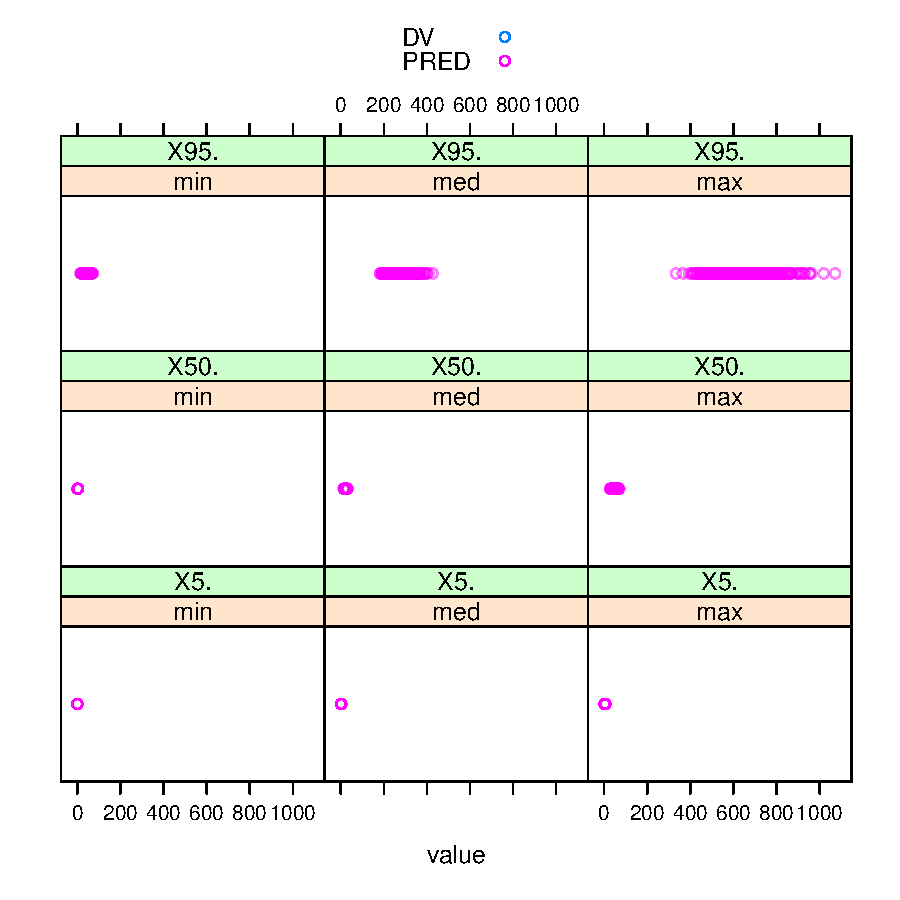
\includegraphics{model-stripplot}
\subsubsection{Diamondback: reference regions on density strips}
Here we show the distribution data as density strips, and indicate reference 
regions around the point estimates. Here is one option. Also try swapping `quant' and 
`metric'.
\begin{Schunk}
\begin{Sinput}
> print(stripplot(
+ 	quant~value|metric,
+ 	molten,
+ 	groups=variable,
+ 	auto.key=TRUE,
+ 	panel=panel.stratify,
+ 	alpha=0.5,
+ 	layout=c(1,3),
+ 	scales=list(relation='free'),
+ 	panel.levels = function(x,y,group.number,col,col.line,fill,font,...){
+ 		if(group.number==1)for(d in seq(length.out=length(x))) panel.polygon(
+ 			x=x[[d]]*c(0.8,1,1.25,1),
+ 			y=y[[d]] + c(0.25,0,0.25,0.5),
+ 			border=col.line,
+ 			col=fill,
+ 			...
+ 		)
+ 		else panel.densitystrip(x=x,y=y,col=fill,border=col.line,...)
+ 	}
+ ))
\end{Sinput}
\end{Schunk}
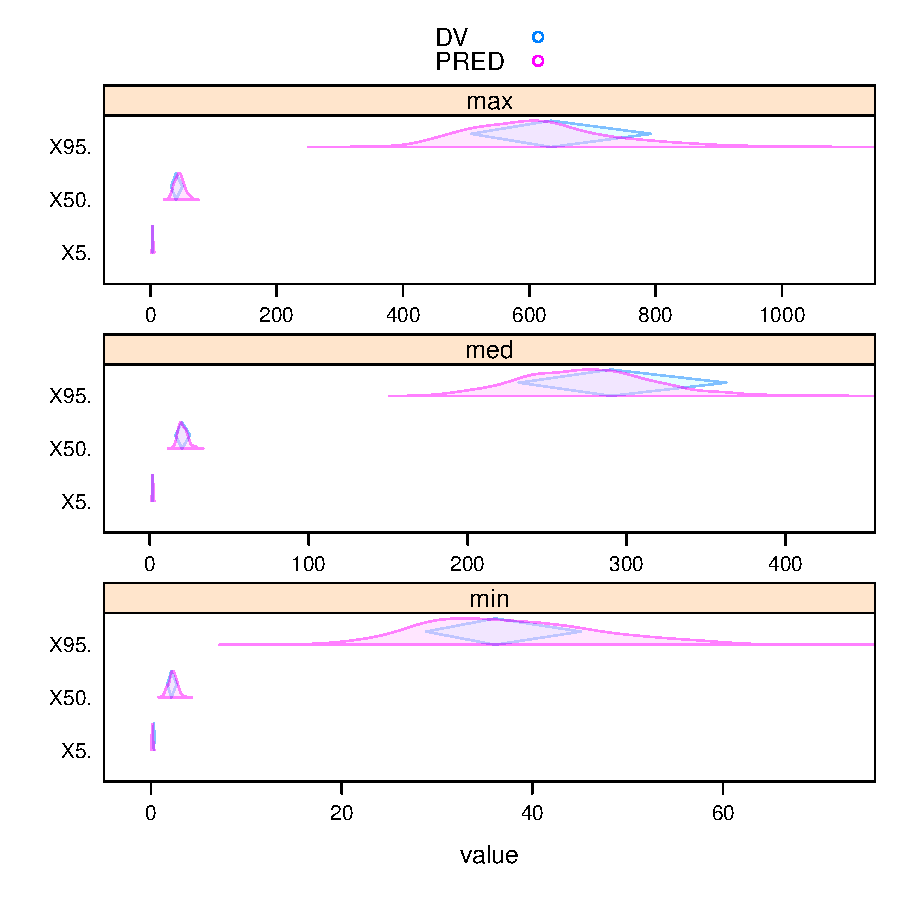
\includegraphics{model-diamondBack}
\section{Bootstrap Estimates of Parameter Uncertainty}
\subsection{Create directories.}
\begin{Schunk}
\begin{Sinput}
> getwd()
\end{Sinput}
\begin{Soutput}
[1] "/Users/timb/project/metrum-mifuns/inst/sample/script"
\end{Soutput}
\begin{Sinput}
> dir.create('../nonmem/1005.boot')
> dir.create('../nonmem/1005.boot/data')
> dir.create('../nonmem/1005.boot/ctl')
\end{Sinput}
\end{Schunk}
\subsection{Create replicate control streams.}
\begin{Schunk}
\begin{Sinput}
> t <- metaSub(
+      clear(readLines('../nonmem/ctl/1005.ctl'),';.+',fixed=FALSE),
+      names=1:300,
+      pattern=c(
+          '1005',
+          '../../data/derived/phase1.csv',
+          '$COV',
+          '$TABLE'
+      ),
+      replacement=c(
+          '*',
+          '../data/*.csv',
+          ';$COV',
+          ';$TABLE'
+     ),
+     fixed=TRUE,
+     out='../nonmem/1005.boot/ctl',
+     suffix='.ctl'
+  )
\end{Sinput}
\end{Schunk}
\subsection{Create replicate data sets by resampling original.}
\begin{Schunk}
\begin{Sinput}
>  bootset <- read.csv('../data/derived/phase1.csv')
>  r <- resample(
+  	bootset,
+  	names=1:300,
+  	key='ID',
+  	rekey=TRUE,
+  	out='../nonmem/1005.boot/data',
+  	stratify='SEX'
+  )
\end{Sinput}
\end{Schunk}
\subsection{Run bootstrap models.}
To force a re-run of bootstraps, delete log.csv.
\begin{Schunk}
\begin{Sinput}
> if(!file.exists('../nonmem/1005.boot/CombRunLog.csv'))NONR(
+      run=1:300,
+      command=command,
+      project='../nonmem/1005.boot/',
+      boot=TRUE,
+      nice=TRUE,
+      streams='../nonmem/1005.boot/ctl'
+ )
> getwd()  
\end{Sinput}
\begin{Soutput}
[1] "/Users/timb/project/metrum-mifuns/inst/sample/script"
\end{Soutput}
\end{Schunk}
\subsection{Summarize bootstrap models.}
When the bootstraps are complete, we return here and summarize. If you 
do not have time for bootstraps, use read.csv() on ../nonmem/1005.boot/log.csv.
\begin{Schunk}
\begin{Sinput}
> #boot <- read.csv('../nonmem/1005.boot/log.csv',as.is=TRUE)
> #wait for bootstraps to finish
> while(!(all(file.exists(paste(sep='','../nonmem/1005.boot/',1:300,'.boot/',1:300,'.lst'))))){}